\documentclass[a4paper,12pt]{article} % добавить leqno в [] для нумерации слева
\usepackage[a4paper,top=1.3cm,bottom=2cm,left=1.5cm,right=1.5cm,marginparwidth=0.75cm]{geometry}
%%% Работа с русским языком
\usepackage{cmap}					% поиск в PDF
\usepackage{mathtext} 				% русские буквы в фомулах
\usepackage[T2A]{fontenc}			% кодировка
\usepackage[utf8]{inputenc}			% кодировка исходного текста
\usepackage[english,russian]{babel}	% локализация и переносы

\usepackage{graphicx}
\usepackage{mathtools}
\usepackage{wrapfig}
\usepackage{tabularx}
\usepackage{amssymb}
\usepackage{hyperref}
\usepackage[rgb]{xcolor}
\hypersetup{colorlinks=true,urlcolor=blue}
%% Шрифты
\usepackage{euscript}	 % Шрифт Евклид
\usepackage{amsmath}
\usepackage{mathtools}
%%% Заголовок
\author{Lokhmatov Arseniy}
\title{Лабораторная работа по общей физике}

\date{\today}
\begin{document}
\begin{titlepage}
    \newpage
    \begin{center}
    {\large МОСКОВСКИЙ ФИЗИКО-ТЕХНИЧЕСКИЙ ИНСТИТУТ (НАЦИОНАЛЬНЫЙ ИССЛЕДОВАТЕЛЬСКИЙ УНИВЕРСИТЕТ)}
    \vspace{1cm}

    {\largeФизтех-школа аэрокосмических технологий}
    \vspace{6em}
    \end{center}
    
    \vspace{1.2em}

    \begin{center}
    %\textsc{\textbf{}}
    \Large Лабораторная работа №3.5.1 \\
    Изучение плазмы газового разряда в неоне
    \linebreak
    \end{center}
    
    \vspace{11em}
    
    \begin{flushright}
                       {\large Работу выполнил\\
                       Лохматов Арсений Игоревич\\
                       Козярский Алексей Сергеевич\\
                       Б03-303 }
    \end{flushright}

    \vspace{\fill}

    \begin{center}
        
\includegraphics[width=0.2\linewidth]{dasr.png}
    \end{center}

    \begin{center}
    Долгопрудный, 2024
    \end{center}

    \end{titlepage}

\section{Теоретическая часть}

\paragraph{Оборудование:} стеклянная газоразрядгая трубка, наполненная неоном, высоковольтный источник питания, источник питания постоянного тока, делитель напряжения, резистор, потенциометр, амперметры, вольтметры, переключатели.

\subsection{Экспериментальная установка}

Схема установки исследования плазмы газового разряда в неоне изображена на рисунке \ref{img1}. Стеклянная газорязрядная трубка имеет ненагреваемый полый катод, который остаётся холодным, три анода и геттерный узел - стеклянный баллон, на внутреннюю поверхность которого напылена газопоглощающая плёнка (геттер). Трубка наполнена изотопом неона $^{22}{Ne}$ при давлении $2$ мм рт. ст. Катод и один из анодов ($I$ или $II$) с помощью переключателя $\text{П}_1$ подкючается через балластный резистор $R_6$ $(\sim 450 \text{ кОм})$ к регулируемому высоковольтному источнику питания $(\text{ВИП})$ с выходным напряжением до $5 \text{ кВ}$.

\begin{figure}[h]
\begin{center}
		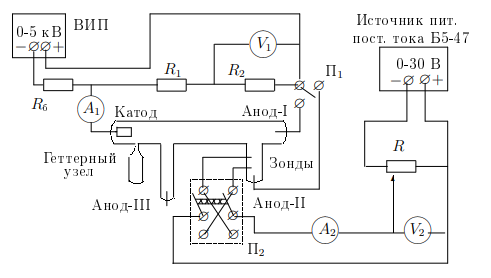
\includegraphics[width=18cm]{card_1.png}
\end{center}
	\caption{Схема установки}
	\label{img1}
\end{figure}

При подключении к $(\text{ВИП})$ анода-I между ним и катодом возникает газовый разряд. Ток разряда измеряется миллиамперметром $A_1$, а падение напряжения на разрядной трубке -- цифровым вольтметром $V_1$, подключённым к трубке через высокоомный $(25 \text{ МОм})$ делитель напржения с коэффициентом $(R_1+R_2)/R_2 = 10$.

Пи подключении к $(\text{ВИП})$ анода-II разряд возникает в пространстве между катодом и анодом-II, где находится двойной зонд, используемый для диагностики плазмы положительного столба.

Зонды изготовлены из молибденовой проволоки диаметром $d=0.2 \text{ мм}$ и имеют длину $l = 5.2 \text{ мм}$. Они подключены к источнику питания $GPS$ через потенциометр $R$. Переключаетль $\text{П}_2$ позволяет изменять полярность напряжения на зондах. Величина напряжения на зондах измеряется с помощью дискретного переключателя $V$ выходного напряжения источника питания и потенциометра $R$, а измеряется цифровым вольтметром $V_2$ (GDM). Для измерения зондового тока используется мультиметр $A_2$ (GDM). Анод-III в нашей работе не используется.

\section{Задание}

В работе предлагается снять вольт-амперную характеристику тлеющего разряда и зондовые характеристики при разных токах разряда и по результатам измерений рассчитать концентрацию и температуру электронов в плазме, плазменную частоту, поляризационную частоту, поляризационную длину, дебаевский радиус экранирования и степень ионизации.

\subsection{Вольт-амперная характеристика разряда}

\begin{enumerate}
    \item Подготовили приборы к работе: работаем с анодом-I (переключатель на анод-I), выходное напряжение $(\text{ВИП})$ сделали равным нулу (ручка регулирования в крайнем левом положении), включили $(\text{ВИП})$ в сеть. 
    Познакомились с правилами работы с мультиметром.
    Подготовили к работе мультиметр $V_1$: включили его в сеть, установили автоматический режим измерения постоянного напряжения.
    Плавно увеличивая выходное напряжение $(\text{ВИП})$, определили напряжения зажигания разряда $U_{\text{заж}}$.

    \[ U_{\text{заж}} = 242.5 \text{ В} \]

    \item С помощью вольтметра $V_1$ и амперметра $A_1$ сняли вольт-амперную характеристику разряда $I_{\text{р}}(U_{\text{р}})$. Ток разряда $I_{\text{р}}$ изменяли в диапазоне от $0.5 \text{ мА}$ до $5 \text{ мА}$. Провели измерения как при нарастании, так и при убывании тока. Результаты занесли в таблицу \ref{tab1}.

    \begin{table}[h]
	\centering
	\begin{tabular}{|c|c|c|}
            \hline
            \multicolumn{3}{|c|}{$\text{Возрастание тока}$} \\ \hline
		\hline
		& $ I_{\text{р}}, \text{ мА}$ & $ U_{\text{р}}, \text{ В}$ \\ \hline
		1 & 0.5248 & 35.001 \\ \hline
            2 & 0.8153 & 34.249 \\ \hline
            3 & 1.1061 & 33.361 \\ \hline
            4 & 1.4093 & 28.703 \\ \hline
            5 & 1.7078 & 23.956 \\ \hline
            6 & 2.0065 & 21.245 \\ \hline
            7 & 2.3067 & 19.252 \\ \hline
            8 & 2.5994 & 16.597 \\ \hline
            9 & 2.9065 & 15.053 \\ \hline
            10 & 3.2042 & 14.422 \\ \hline
            11 & 3.5090 & 13.444 \\ \hline
            12 & 3.8036 & 12.088 \\ \hline
            13 & 4.1026 & 10.545 \\ \hline
            14 & 4.4092 & 8.942 \\ \hline
            15 & 4.7086 & 7.072 \\ \hline
            16 & 5.0059 & 5.416 \\ \hline
	\end{tabular}
        \begin{tabular}{|c|c|c|}
            \hline
            \multicolumn{3}{|c|}{$\text{Убывние тока}$} \\ \hline
		\hline
		& $ I_{\text{р}}, \text{ мА}$ & $ U_{\text{р}}, \text{ В}$ \\ \hline
		1 & 5.0002 & 5.355 \\ \hline
            2 & 4.7068 & 6.996 \\ \hline
            3 & 4.4015 & 8.811 \\ \hline
            4 & 4.1046 & 10.302 \\ \hline
            5 & 3.8057 & 11.788 \\ \hline
            6 & 3.5096 & 13.134 \\ \hline
            7 & 3.2047 & 14.011 \\ \hline
            8 & 2.9035 & 14.953 \\ \hline
            9 & 2.6062 & 16.361 \\ \hline
            10 & 2.3051 & 18.873 \\ \hline
            11 & 2.0228 & 20.777 \\ \hline
            12 & 1.7033 & 23.792 \\ \hline
            13 & 1.4021 & 28.433 \\ \hline
            14 & 1.1023 & 33.295 \\ \hline
            15 & 0.8065 & 34.378 \\ \hline
            16 & 0.5089 & 35.144 \\ \hline
	\end{tabular}
	\caption{Вольт-амперная характеристика разряда}
	\label{tab1}
    \end{table}
    
\end{enumerate}

\newpage

\subsection{Зондовые характеристики}

\begin{enumerate}
    \item Уменшили напряжение $(\text{ВИП})$ до нуля, переведи переключатель $\text{П}_1$ на анод-II, переключатель $\text{П}_2$ переключили на $+$.
    Подготовили к работе мультиметры $A_2$ и $V_2$, включили приборы в сеть.
    На $A_2$ установили автоматический режим измерения постоянного тока в мкА. На $V_2$ установили автоматический режим измерения напряжения в вольтах.
    \item Плавно увеличивая напряжения $(\text{ВИП})$ до возникновения разряда и установили разрядный ток $I_{\text{р}} \sim 5 \text{ мА}$.
    Включили в сеть источник питания $GPS$, нажали кнопку $OUTPUT$, установили произвольный ток, затем напряжение $U_2 \sim \text{ В}$.
    При помощи потенциометра $R$ установили на зонде максимальное напряжение $U_2 \sim \text{ В}$.
    \item С помощью мультиметров $A_2$ и $V_2$ снимем вольт-амперную характеристику двойного зонда $I_{\text{з}}(U_{\text{з}})$ при фиксированном токе разряда $I_{\text{р}}$.

    Проделаем теже действия при токах разряда, равных $3$ и $1.5 \text{ мА}$. Результаты занесём в таблицу \ref{tab2}.

    \begin{table}[h]
	\centering
	\begin{tabular}{|c|c|c|}
            \hline
            \multicolumn{3}{|c|}{$I_\text{р} = 5 \text{ мВ}$} \\ \hline
		\hline
		& $ U_{\text{з}}, \text{ мА}$ & $ I_{\text{з}}, \text{ В}$ \\ \hline
		1 & 25.013 & 109.24 \\ \hline
            2 & 22.085 & 107.02 \\ \hline
            3 & 19.062 & 103.55 \\ \hline
            4 & 16.024 & 97.79 \\ \hline
            5 & 13.004 & 88.89 \\ \hline
            6 & 10.258 & 77.93 \\ \hline
            7 & 8.066 & 67.42 \\ \hline
            8 & 6.077 & 56.33 \\ \hline
            9 & 4.1406 & 44.93 \\ \hline
            10 & 2.0787 & 30.42 \\ \hline
            11 & 0.0007 & 12.93 \\ \hline
            12 & -0.0020 & -11.70 \\ \hline
            13 & -2.0112 & -27.06 \\ \hline
            14 & -4.1820 & -43.05 \\ \hline
            15 & -6.106 & -55.27 \\ \hline
            16 & -8.051 & -66.53 \\ \hline
            17 & -10.085 & -77.62 \\ \hline
            18 & -13.071 & -91.03 \\ \hline
            19 & -16.078 & -101.64 \\ \hline
            20 & -19.096 & -109.30 \\ \hline
            21 & -22.175 & -114.04 \\ \hline
            22 & -25.018 & -116.71 \\ \hline
	\end{tabular}
        \begin{tabular}{|c|c|c|}
            \hline
            \multicolumn{3}{|c|}{$I_\text{р} = 3 \text{ мВ}$} \\ \hline
		\hline
		& $ U_{\text{з}}, \text{ мА}$ & $ I_{\text{з}}, \text{ В}$ \\ \hline
		1 & 24.821 & 64.989 \\ \hline
            2 & 22.102 & 63.009 \\ \hline
            3 & 19.085 & 61.079 \\ \hline
            4 & 16.012 & 58.708 \\ \hline
            5 & 13.061 & 55.042 \\ \hline
            6 & 9.989 & 48.482 \\ \hline
            7 & 8.064 & 42.235 \\ \hline
            8 & 6.052 & 33.997 \\ \hline
            9 & 3.991 & 23.381 \\ \hline
            10 & 2.091 & 12.038 \\ \hline
            11 & 0.002 & 1.008 \\ \hline
            12 & -0.041 & -7.004 \\ \hline
            13 & -2.075 & -20.21 \\ \hline
            14 & -4.083 & -32.16 \\ \hline
            15 & -6.124 & -42.46 \\ \hline
            16 & -8.099 & -50.47 \\ \hline
            17 & -10.047 & -56.66 \\ \hline
            18 & -13.031 & -63.23 \\ \hline
            19 & -16.082 & -67.24 \\ \hline
            20 & -19.186 & -69.82 \\ \hline
            21 & -22.134 & -71.78 \\ \hline
            22 & -25.016 & -73.69 \\ \hline
	\end{tabular}
        \begin{tabular}{|c|c|c|}
            \hline
            \multicolumn{3}{|c|}{$I_\text{р} = 1.5 \text{ мВ}$} \\ \hline
		\hline
		& $ U_{\text{з}}, \text{ мА}$ & $ I_{\text{з}}, \text{ В}$ \\ \hline
		1 & 25.077 & 32.33 \\ \hline
            2 & 22.044 & 31.24 \\ \hline
            3 & 19.114 & 30.20 \\ \hline
            4 & 16.133 & 29.08 \\ \hline
            5 & 13.087 & 27.45 \\ \hline
            6 & 10.081 & 24.59 \\ \hline
            7 & 8.025 & 21.55 \\ \hline
            8 & 6.083 & 17.64 \\ \hline
            9 & 4.094 & 12.44 \\ \hline
            10 & 2.121 & 6.06 \\ \hline
            11 & 0.03 & 0.87 \\ \hline
            12 & -0.032 & -5.003 \\ \hline
            13 & -2.087 & -10.31 \\ \hline
            14 & -3.992 & -16.58 \\ \hline
            15 & -6.143 & -22.26 \\ \hline
            16 & -8.022 & -26.27 \\ \hline
            17 & -10.017 & -29.37 \\ \hline
            18 & -13.054 & -32.55 \\ \hline
            19 & -16.079 & -34.42 \\ \hline
            20 & -19.043 & -35.76 \\ \hline
            21 & -22.092 & -37.07 \\ \hline
            22 & -25.033 & -38.85 \\ \hline
	\end{tabular}
	\caption{Зондовая характеристика}
	\label{tab2}
    \end{table}
    
    \item Перевели ручки регулировки источника питания к минимальным значениями отключим приборы. Запишем параметры зондов.

    \[ d = 0.2 \text{ мм}; \text{ } l = 5.2 \text{ мм} \]
\end{enumerate}

\newpage

\subsection{Обработка результатов}

\begin{enumerate}
    \item Построим вольт-амперную характеристику разряда в координатах $I_{\text{р}}(U_{\text{р}})$.

    \begin{figure}[h]
        \begin{center}
    		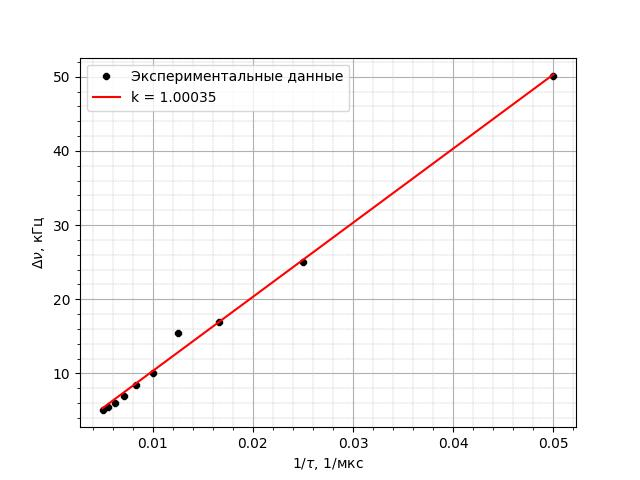
\includegraphics[width=16cm]{image1.jpg}
        \end{center}
        \caption{График зависимости $I_{\text{р}}(U_{\text{р}})$ на повышении напряжения}
        \label{plot1}
    \end{figure}

    \[ R_{\text{диф}} = \frac{\text{dU}}{\text{dI}} = \frac{1}{k}, \text{ } \sigma_{R} = R \frac{\sigma_{k}}{k} \]
    \[ k_{1} = -(0.01846 \pm 0.00044) \text{ } \frac{\text{мА}}{\text{В}} \text{ } \Longrightarrow R_{max} = -\frac{1}{0.01846 \cdot 10^{-3}} = -(5.42 \pm 0.13) \text{ } \cdot 10^{4} \text{ Ом} \text{ } (\varepsilon=2.38\%) \]
    \[ k_{2} = -(0.00640 \pm 0.00006) \text{ } \frac{\text{мА}}{\text{В}} \text{ } \Longrightarrow R_{min} = -\frac{1}{0.0064 \cdot 10^{-3}} = -(15.63 \pm 0.15) \text{ } \cdot 10^{4} \text{ Ом} \text{ } (\varepsilon=0.94\%) \]

    \newpage

    \begin{figure}[h]
        \begin{center}
    		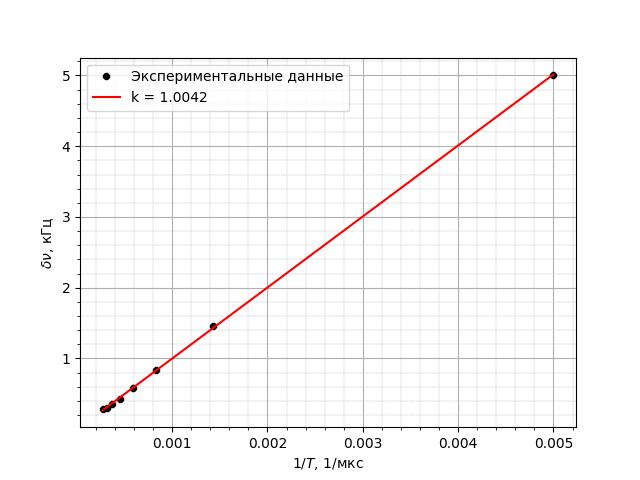
\includegraphics[width=16cm]{image2.jpg}
        \end{center}
        \caption{График зависимости $I_{\text{р}}(U_{\text{р}})$ на понижении напряжения}
        \label{plot2}
    \end{figure}

    \[ k_{3} = -(0.02001 \pm 0.00006) \text{ } \frac{\text{мА}}{\text{В}} \text{ } \Longrightarrow R_{max} = -\frac{1}{0.02001 \cdot 10^{-3}} = -(4.99 \pm 0.02) \text{ } \cdot 10^{4} \text{ Ом} \text{ } (\varepsilon=0.29\%) \]
    \[ k_{4} = -(0.00717 \pm 0.0006) \text{ } \frac{\text{мА}}{\text{В}} \text{ } \Longrightarrow R_{min} = -\frac{1}{0.00717 \cdot 10^{-3}} = -(13.95 \pm 1.17) \text{ } \cdot 10^{4} \text{ Ом} \text{ } (\varepsilon=8.37\%) \]

    \newpage

    \item Построим зондовые характеристики для разных токов разряда, отцентрируем кривыеи и используем их для определения температуры электронов $T_{e}$.

    \[ kT_{e} = \frac{1}{2}\frac{eI_{i\text{н}}}{\frac{dI}{dU}|_{U=0}}, \text{ } kT_{e} = \frac{\Delta U}{2} \]
    
    Оценим погрешности.
    
    \[ \sigma_{kT_{e}} = (kT_{e})\sqrt{\left(\frac{\sigma_{I_{i}}}{I_{i}}\right)^2 + \left(\frac{\sigma_{\frac{dI}{dU}}}{\frac{dI}{dU}}\right)^2}, \text{ } \sigma_{kT_{e}} = (kT_{e})\frac{\sigma_{\Delta U}}{\Delta U} \]

    \begin{figure}[h]
        \begin{center}
    		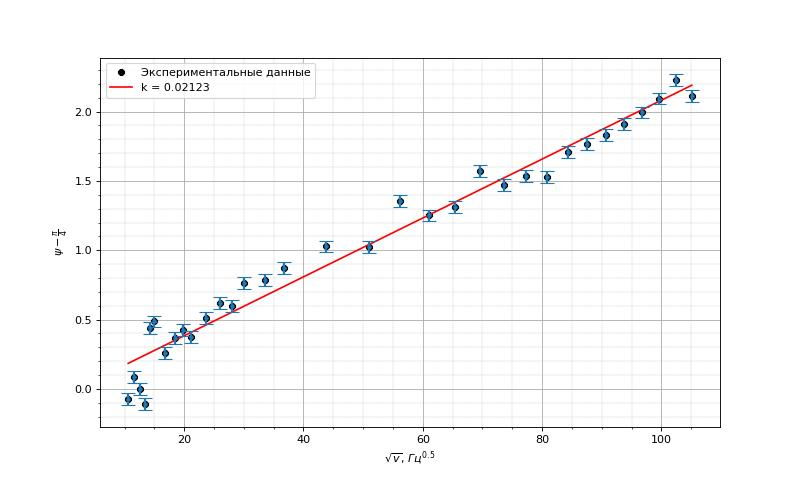
\includegraphics[width=15cm]{image3.jpg}
        \end{center}
        \caption{Зондовая характеристика $I_{\text{раз}}=5 \text{ мА}$}
        \label{plot3}
    \end{figure}

    \begin{table}[h]
	\centering
	\begin{tabular}{|c|c|c|c|c|c|c|c|}
            \hline
            $I_{i_\text{сред}}, \text{ мкА}$ & $\sigma_{I_{i}}, \text{ мкА}$ & $\Delta U_{\text{сред}}, \text{ В}$ & $\sigma_{\Delta U}, \text{ В}$ & $\frac{dI}{dU}|_{U=0}, \text{ }\frac{\text{мкА}}{\text{В}}$ & $\sigma, \text{ }\frac{\text{мкА}}{\text{В}}$ \\ \hline
            73.235 & 3.169 & 9.1 & 0.01 & 8 & 0.01 \\ \hline
            $(kT_{e})_1, \text{ эВ}$ & $\sigma_{kT_{e}}, \text{ эВ}$ & $(kT_{e})_2, \text{ эВ}$ & $\sigma_{kT_{e}}, \text{ эВ}$ & $T_1, \cdot 10^3 \text{ К}$ & $T_2, \cdot 10^3 \text{ К}$ \\ \hline
            4.58 & 0.21 & 4.550 & 0.005 & 53.101 & 52.754  \\ \hline
	\end{tabular}
	\caption{Результаты вычислений}
	\label{tab3}
    \end{table}

    \newpage

    \begin{figure}[h]
        \begin{center}
    		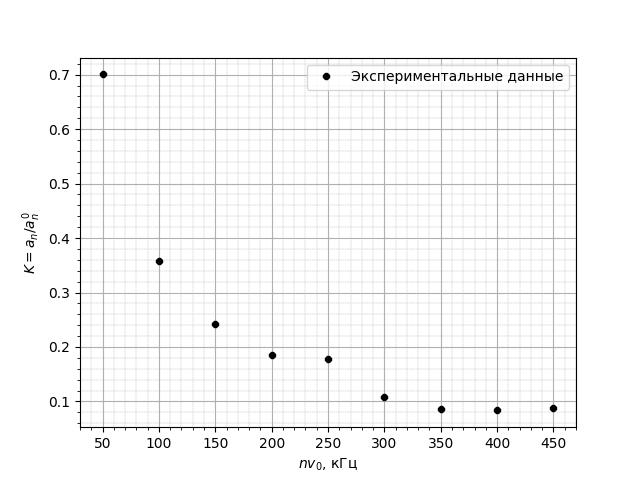
\includegraphics[width=15cm]{image4.jpg}
        \end{center}
        \caption{Зондовая характеристика $I_{\text{раз}}=3 \text{ мА}$}
        \label{plot4}
    \end{figure}

    \begin{table}[h]
	\centering
	\begin{tabular}{|c|c|c|c|c|c|c|c|}
            \hline
            $I_{i_\text{сред}}, \text{ мкА}$ & $\sigma_{I_{i}}, \text{ мкА}$ & $\Delta U_{\text{сред}}, \text{ В}$ & $\sigma_{\Delta U}, \text{ В}$ & $\frac{dI}{dU}|_{U=0}, \text{ }\frac{\text{мкА}}{\text{В}}$ & $\sigma, \text{ }\frac{\text{мкА}}{\text{В}}$ \\ \hline
            48.560 & 0.289 & 7.25 & 0.01 & 6.5 & 0.01 \\ \hline
            $(kT_{e})_1, \text{ эВ}$ & $\sigma_{kT_{e}}, \text{ эВ}$ & $(kT_{e})_2, \text{ эВ}$ & $\sigma_{kT_{e}}, \text{ эВ}$ & $T_1, \cdot 10^3 \text{ К}$ & $T_2, \cdot 10^3 \text{ К}$ \\ \hline
            3.741 & 0.023 & 3.625 & 0.005 & 43.374 & 42.029 \\ \hline
	\end{tabular}
	\caption{Результаты вычислений}
	\label{tab4}
    \end{table}

    \newpage

    \begin{figure}[h]
        \begin{center}
    		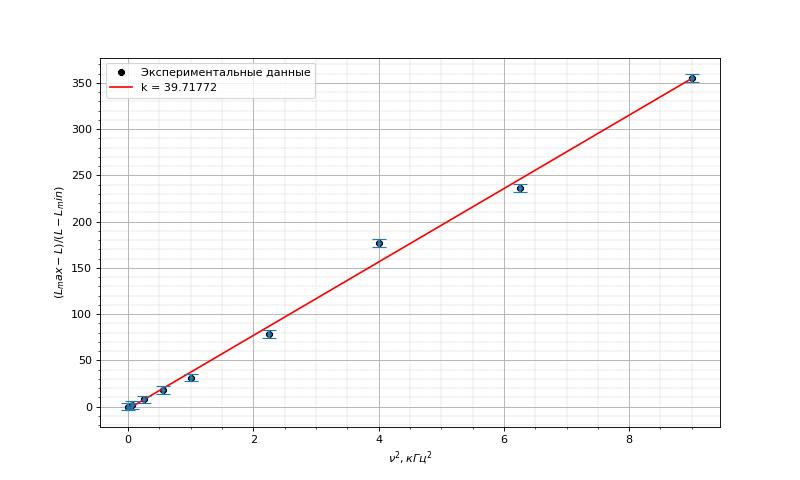
\includegraphics[width=15cm]{image5.jpg}
        \end{center}
        \caption{Зондовая характеристика $I_{\text{раз}}=1.5 \text{ мА}$}
        \label{plot5}
    \end{figure}

    \begin{table}[h]
	\centering
	\begin{tabular}{|c|c|c|c|c|c|c|c|}
            \hline
            $I_{i_\text{сред}}, \text{ мкА}$ & $\sigma_{I_{i}}, \text{ мкА}$ & $\Delta U_{\text{сред}}, \text{ В}$ & $\sigma_{\Delta U}, \text{ В}$ & $\frac{dI}{dU}|_{U=0}, \text{ }\frac{\text{мкА}}{\text{В}}$ & $\sigma, \text{ }\frac{\text{мкА}}{\text{В}}$ \\ \hline
            21.68 & 0.58 & 7.2 & 0.01 & 3 & 0.01 \\ \hline
            $(kT_{e})_1, \text{ эВ}$ & $\sigma_{kT_{e}}, \text{ эВ}$ & $(kT_{e})_2, \text{ эВ}$ & $\sigma_{kT_{e}}, \text{ эВ}$ & $T_1, \cdot 10^3 \text{ К}$ & $T_2, \cdot 10^3 \text{ К}$ \\ \hline
            3.612 & 0.097 & 3.600 & 0.005 & 41.878 & 41.739  \\ \hline
	\end{tabular}
	\caption{Результаты вычислений}
	\label{tab5}
    \end{table}

    \newpage

    \item Построим на одном листе Семейство отцентрованных зондовых характеристик $I_\text{з}(U_\text{з})$.
    \begin{figure}[h]
        \begin{center}
    		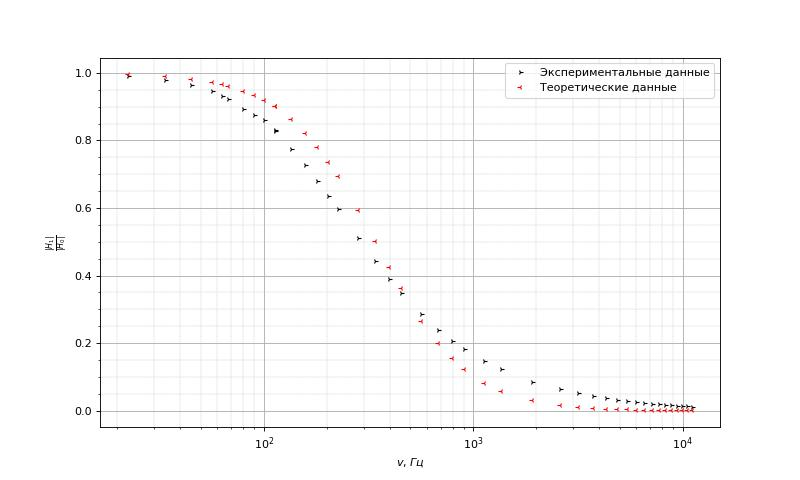
\includegraphics[width=15cm]{image6.jpg}
        \end{center}
        \caption{Семейство отцентрованных зондовых характеристик $I_\text{з}(U_\text{з})$}
        \label{plot6}
    \end{figure}

    \item Полагая $n_e=n_i=n$, найдём эту концентрацию, используя формулу Бома:

    \[ I_{i\text{н}}=0.4n_{e}eS\sqrt{\frac{2kT_{e}}{m_{i}}}, \] \[ \text{ где } S=\pi\cdot d\cdot l = \pi \cdot 0.2 \cdot 5.2 \cdot 10^{-6} = 3.27 \cdot 10^{-6} \text{ м}^2 \text{ -- площадь поверхности зонда; } \] \[ m_{i} = 22\cdot 1.66 \cdot 10^{-27} \text{ кг -- масса иона неона.} \]

    \[ \Longrightarrow n_{e} = \frac{I_{i\text{н}}}{0.4eS}\sqrt{\frac{m_{i}}{2kT_{e}}}; \text{ } \sigma_{n_e} = n_e\sqrt{\left(\frac{\sigma_{I_{i\text{н}}}}{I_{i\text{н}}}\right)^2 + \left(\frac{1}{2}\frac{\sigma_{T_e}}{T_e}\right)^2} \]

    \begin{table}[h]
	\centering
	\begin{tabular}{|c|c|c|c|c|c|c|}
            \hline
            $I_{\text{разр}}, \text{ мА}$ & $I_{i_\text{н}}, \text{ мкА}$ & $\sigma_{I_{i\text{н}}}, \text{ мкА}$ & $T_e, \cdot 10^3 \text{ К}$ & $\sigma_{T_e}, \cdot 10^3 \text{ К}$ & $n_e, \cdot 10^{16} \text{ }\frac{\text{част}}{\text{м}^3}$ & $\sigma_{n_e}, \cdot 10^{16} \text{ }\frac{\text{част}}{\text{м}^3}$  \\ \hline
            5 & 73.235 & 3.169 & 52.928 & 0.058 & 5.533 & 0.239 \\ \hline
            3 & 48.560 & 0.289 & 42.702 & 0.059 & 4.084 & 0.024 \\ \hline
            1.5 & 21.68 & 0.58 & 41.809 & 0.058 & 1.843 & 0.049 \\ \hline
	\end{tabular}
	\caption{Результаты вычислений}
	\label{tab6}
    \end{table}

    \item Рассчитаем плазменную частоту колебаний электронов по формуле

    \[ \omega_{p} = \sqrt{\frac{4\pi n_e e^2}{m_e}} = 5.6\cdot 10^{4}\sqrt{n_e} \text{ }\frac{\text{рад}}{\text{сек}};  \sigma_{\omega_p} = \omega_p \frac{1}{2}\frac{\sigma_{n_e}}{n_e} \]

    Через такую плазму при падении на неё электромагнитного излучения пройдут только те частоты, которые больше плазменной.

    \begin{table}[h]
	\centering
	\begin{tabular}{|c|c|c|c|c|}
            \hline
            $I_{\text{разр}}, \text{ мА}$ & $n_e, \cdot 10^{16} \text{ }\frac{\text{част}}{\text{м}^3}$ & $\sigma_{n_e}, \cdot 10^{16} \text{ }\frac{\text{част}}{\text{м}^3}$ & $\omega_{p}, \cdot 10^{13} \text{ }\frac{\text{рад}}{\text{сек}}$ & $\sigma_{\omega_{p}}, \cdot 10^{13} \text{ }\frac{\text{рад}}{\text{сек}}$  \\ \hline
            5 & 5.533 & 0.239 & 1.317 & 0.028 \\ \hline
            3 & 4.084 & 0.024 & 1.132 & 0.003 \\ \hline
            1.5 & 1.843 & 0.049 & 0.760 & 0.010 \\ \hline
	\end{tabular}
	\caption{Результаты вычислений}
	\label{tab7}
    \end{table}

    Рассчитаем электронную поляризационную длину $r_{D_e}$ по формуле

    \[ r_{D_e }= \sqrt{\frac{kT_e}{4\pi n_e e^2}}; \text{ } \sigma_{r_{D_e}} = r_{D_e} \sqrt{\left(\frac{1}{2}\frac{\sigma_{T_e}}{T_e}\right)^2 + \left(\frac{1}{2}\frac{\sigma_{n_e}}{n_e}\right)^2 } \]

    \begin{table}[h]
	\centering
	\begin{tabular}{|c|c|c|c|c|c|c|}
            \hline
            $I_{\text{разр}}, \text{ мА}$ & $T_e, \cdot 10^3 \text{ К}$ & $\sigma_{T_e}, \cdot 10^3 \text{ К}$ & $n_e, \cdot 10^{16} \text{ }\frac{\text{част}}{\text{м}^3}$ & $\sigma_{n_e}, \cdot 10^{16} \text{ }\frac{\text{част}}{\text{м}^3}$ & $ r_{D_e}, \text{ мкм}$ & $ \sigma{r_{D_e}}, \text{ мкм}$  \\ \hline
            5 &  52.928 & 0.058 & 5.533 & 0.239 & 6.408 & 0.138 \\ \hline
            3 &  42.702 & 0.059 & 4.084 & 0.024 & 6.697 & 0.020 \\ \hline
            1.5 & 41.809 & 0.058 & 1.843 & 0.049 & 9.865 & 0.131 \\ \hline
	\end{tabular}
	\caption{Результаты вычислений}
	\label{tab8}
    \end{table}

    Поскольку электронная поляризационная длина намного меньше линейныз размеров плазмы, поэтому мы можем считать её \textbf{квазинейтральной}.

    Рассчитаем дебаевский радиус экранирования $r_{D}$, используя следующую формулу, где $T_{e} \gg T{i}$, а температура ионов равно комнатной ($T{i} = 300 K$)

    \[ r_{D} = \sqrt{\frac{kT_{i}}{4\pi n_{e}e^2}}, \text{ } \sigma_{r_D} = r_{D}\frac{1}{2}\frac{\sigma_{n_e}}{n_e} \]

    \begin{table}[h]
	\centering
	\begin{tabular}{|c|c|c|c|c|}
            \hline
            $I_{\text{разр}}, \text{ мА}$ & $n_e, \cdot 10^{16} \text{ }\frac{\text{част}}{\text{м}^3}$ & $\sigma_{n_e}, \cdot 10^{16} \text{ }\frac{\text{част}}{\text{м}^3}$ & $r_D, \text{ мкм}$ & $\sigma_{r_d}, \text{ мкм}$  \\ \hline
            5 & 5.533 & 0.239 & 4.82 & 0.11 \\ \hline
            3 & 4.084 & 0.024 & 5.60 & 0.01 \\ \hline
            1.5 & 1.843 & 0.049 & 8.35 & 0.01 \\ \hline
	\end{tabular}
	\caption{Результаты вычислений}
	\label{tab9}
    \end{table}

    \item Оценим среднее число ионов в дебаевской сфере

    \[ N_{D} = \frac{4}{3}\pi r_{d}^3 n_{i}; \text{ } \sigma_{N_D} = N_{D}\sqrt{\left(3\cdot\frac{\sigma_{r_D}}{r_{D}}\right)^2 + \left(\frac{\sigma_{n_i}}{n_{i}}\right)^2} \]

    \newpage

    \begin{table}[h]
	\centering
	\begin{tabular}{|c|c|c|c|c|c|c|}
            \hline
            $I_{\text{разр}}, \text{ мА}$ & $n_e, \cdot 10^{16} \text{ }\frac{\text{част}}{\text{м}^3}$ & $\sigma_{n_e}, \cdot 10^{16} \text{ }\frac{\text{част}}{\text{м}^3}$ & $r_D, \text{ мкм}$ & $\sigma_{r_d}, \text{ мкм}$ & $N_{D}$ & $\sigma_{N_D}$  \\ \hline
            5 & 5.533 & 0.239 & 4.82 & 0.11 & 26 & 2 \\ \hline
            3 & 4.084 & 0.024 & 5.60 & 0.01 & 30 & 0 \\ \hline
            1.5 & 1.843 & 0.049 & 8.35 & 0.01 & 45 & 1 \\ \hline
	\end{tabular}
	\caption{Результаты вычислений}
	\label{tab10}
    \end{table}

    Поскольку мы получили, что $N_{D} \gg 1$, то есть выполняется условие идеальной плазмы, то нашу плазму можно считать \textbf{идеальной}.

    \item Оценим степень ионизации плазмы (долю ионизированных атомов $\alpha$), если давление в трубке $P=2\text{ торр}$: $\alpha = n_{i}/n$, где $n$ -- общее число частиц в единицу объёма.

    \[ P=nkT_{i} \longleftrightarrow n = \frac{P}{kT_{i}}; \text{ } \sigma_n = n\frac{\sigma_{T_i}}{T_i} \]

    \begin{table}[h]
	\centering
	\begin{tabular}{|c|c|c|c|c|c|c|c|}
            \hline
            $I_{\text{разр}}, \text{ мА}$ & $T_e, \cdot 10^3 \text{ К}$ & $n_e, \cdot 10^{16} \text{ }\frac{\text{част}}{\text{м}^3}$ & $\sigma_{n_e}, \cdot 10^{16} \text{ }\frac{\text{част}}{\text{м}^3}$ & $ n, \cdot 10^{20} $ & $ \sigma_{n}, \cdot 10^{20} $ & $\alpha,  \cdot 10^{-4}$ & $\sigma_{\alpha},  \cdot 10^{-4}$  \\ \hline
            5 &  52.928 & 5.533 & 0.239 & 3.656 & 0.004 & 1.513 & 0.065 \\ \hline
            3 &  42.702 & 4.084 & 0.024 & 4.531 & 0.006 & 0.901 & 0.005 \\ \hline
            1.5 & 41.809 & 1.843 & 0.049 & 4.628 & 0.006 & 0.398 & 0.011 \\ \hline
	\end{tabular}
	\caption{Результаты вычислений}
	\label{tab11}
    \end{table}

    \item Построим графики ззависимостей электронной температуры и концентрации электронов от тока разряда $T_{e}(I_{\text{р}})$ и $n_{e}(I_{\text{р}})$.

    \begin{figure}[h]
    \begin{center}
    		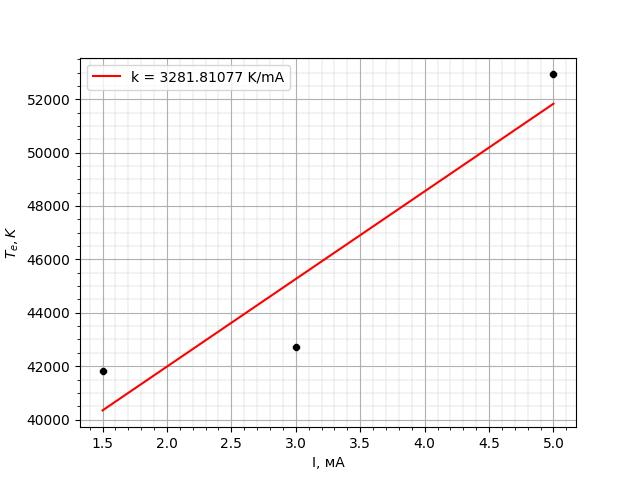
\includegraphics[width=14cm]{image7.jpg}
    \end{center}
    	\caption{График зависимости электронной температуры от тока разряда $T_{e}(I_{\text{р}})$}
    	\label{img7}
    \end{figure}

    \begin{figure}[h]
    \begin{center}
    		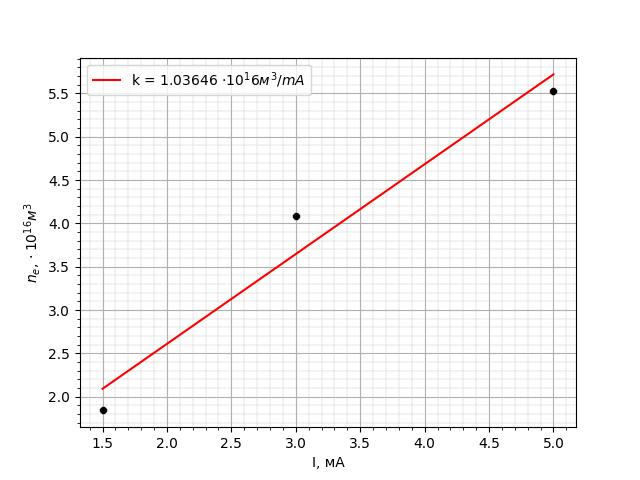
\includegraphics[width=14cm]{image8.jpg}
    \end{center}
    	\caption{График зависимости концентрации электронов от тока разряда $n_{e}(I_{\text{р}})$}
    	\label{img8}
    \end{figure}

     Видим, что скорее всего в обоих случаях зависимость линейная, но по трём точкам сказать точно нельзя!
    
\end{enumerate}

\section{Подведение итогов и выводы}

В этой лабораторной работе мы узучали плазму газового разряда в неоне, проверили свойство квазистатичности плазмы, а так же является ли наша плазма идеальной или нет. 

При разных токах разряда мы определили несколько характеристик плазмы, которые представлены в таблице \ref{tab12}.

    \begin{table}[h]
	\centering
	\begin{tabular}{|c|c|c|c|c|c|c|c|}
            \hline
            $I_{\text{р}}, \text{ мА}$ & $kT_{\text{e}}, \text{ эВ}$ & $n_{\text{e}}, \text{ см}^{-3}$ & $\omega_{\text{p}}, \text{ рад/сек}$ & $r_{D_e}, \text{ см}$ & $r_{D}, \text{ см}$ & $N_{D}$ & $\alpha$ \\ \hline
            5 & 4.58 & 5.533 $\cdot 10^{16}$ & 1.317 $\cdot 10^{13}$ & 6.408 $\cdot 10^{-4}$ & 4.82 $\cdot 10^{-4}$ & 26 & 1.513 $\cdot 10^{-4}$ \\ \hline
            3 & 3.741 & 4.084 $\cdot 10^{16}$ & 1.132 $\cdot 10^{13}$ & 6.697 $\cdot 10^{-4}$ & 5.60 $\cdot 10^{-4}$ & 30 & 0.901 $\cdot 10^{-4}$ \\ \hline
            1.5 & 3.612 & 1.843 $\cdot 10^{16}$ & 0.760 $\cdot 10^{13}$ & 9.865 $\cdot 10^{-4}$ & 8.35 $\cdot 10^{-4}$ & 45 & 0.398 $\cdot 10^{-4}$ \\ \hline
        \end{tabular}
	\caption{Сводная таблица}
	\label{tab12}
    \end{table}

    Полученные результаты совпадают по порядку с табличными. Так же были оценены погрешности найденных величин.

\end{document}
